\chapter{PHYSICS OBJECT RECONSTRUCTION} \label{reco}

In the early days of particle physics experimentation, charged particles were visually identified by analyzing photographs of the ionization tracks left behind in cloud chambers and bubble chambers. Given the higher collision energies and instantaneous luminosities demanded by modern experiments, the amount of information recorded for a collision event renders such visual analyses intractable. The final state particles produced by a proton collision at the LHC are recorded as electronic signals by the CMS detector, and the accurate interpretation of these signals as physics objects is what enables the full reconstruction of the collision's aftermath. The definition and reconstruction of the standard physics objects, with an emphasis on those used by the \VHbb\ analysis, are described in this chapter.

\section{Particle-Flow Reconstruction}

The hermetic design of the CMS detector and the granularity of its subsystems enabled the first successful deployment of a \textit{particle-flow (PF)} based reconstruction algorithm at a hadron collider experiment.\cite{PARTICLEFLOW} Although the individual subsystems are capable of reconstructing the particles for which they were designed, a more accurate and global event description can be achieved by combining the measurements obtained by the subsystems as a whole. Since its commissioning, the PF algorithm has been used online to improve the efficiency of the High-Level Trigger (HLT) and offline to improve the quality of the reconstructed particle candidates considered by physics analyses.

The PF algorithm begins with the basic \textit{elements} produced by each detector subsystem: the silicon tracker and muon chambers both provide charged particle \textit{tracks}, while the electromagnetic calorimeter (ECAL) and hadronic calorimeter (HCAL) both provide \textit{clusters} of absorbed energy. A \textit{link algorithm} which tests the compatibility of pairs of elements from different subsystems is used to generate \textit{blocks} of elements that are directly linked or indirectly linked through common elements. Individual particles are subsequently identified and reconstructed within each block, starting with muons then proceeding to electrons, photons, and charged and neutral hadrons. As particles are reconstructed, the elements associated with that particle are removed from the block such that each particle is reconstructed from a set of unique elements. Once all the blocks have been processed and all particles in the event have been identified and reconstructed, a post-processing algorithm is used to correct misidentified or misreconstructed high-\pT\ muons which can artificially increase the reconstructed missing transverse momentum \pTmiss\ in the event.

\begin{figure}[htbp]
  \centering
    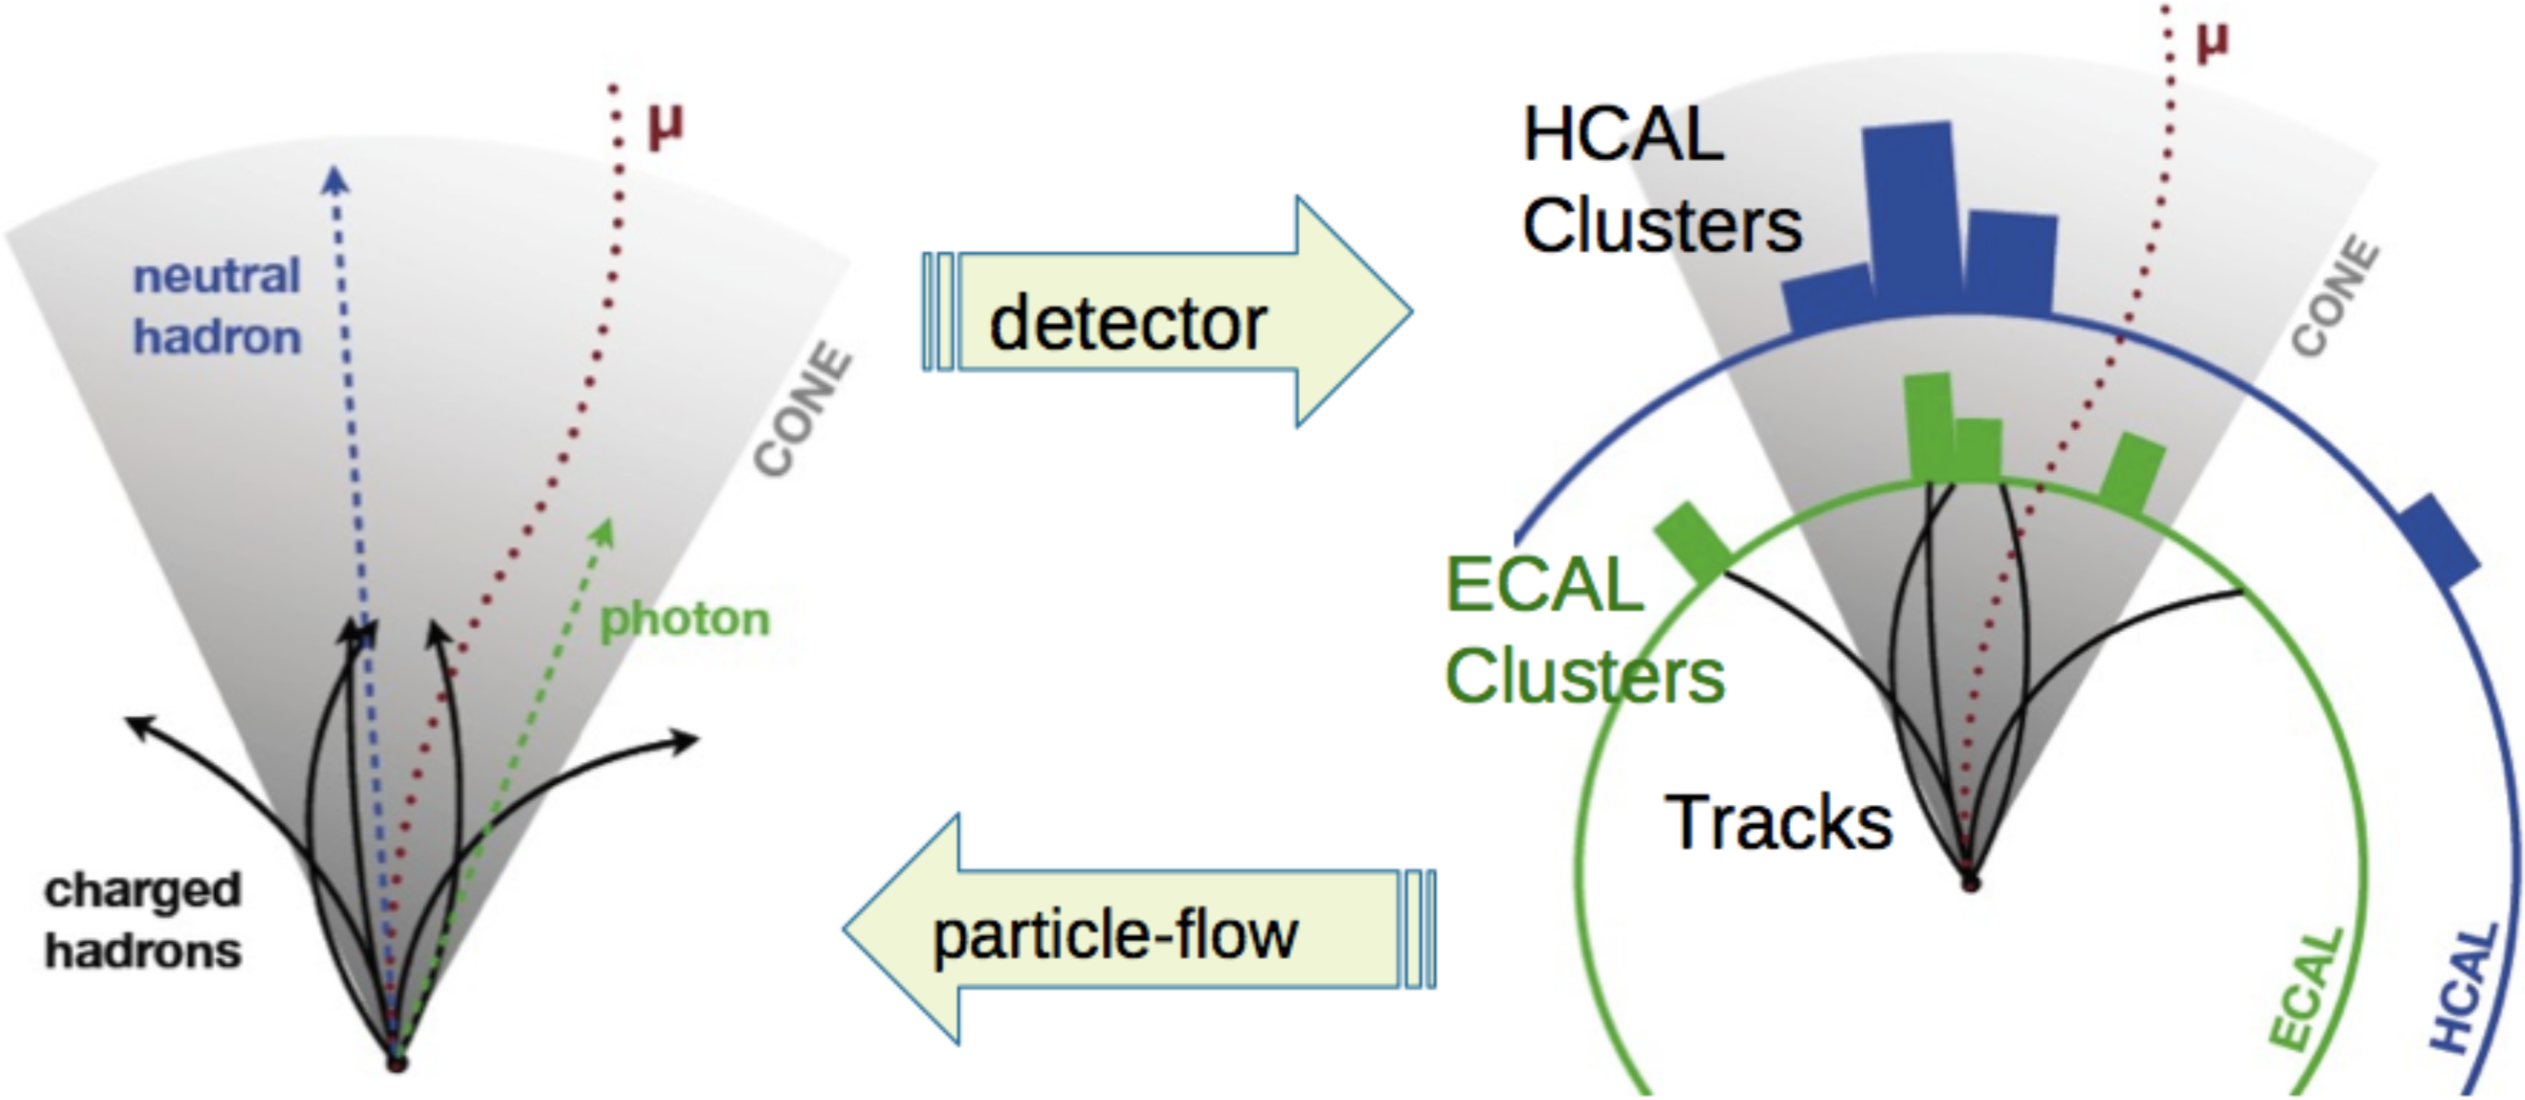
\includegraphics[width=5in]{images/pfdiagram}
    \caption[Particle-Flow Infographic]{An infographic illustrating the particle-flow reconstruction paradigm.\cite{pfdiagram}}
    \label{fig:pfdiagram}
\end{figure}

At this stage, the particle candidates proposed by the PF algorithm are ready to be used in physics analyses. In practice, the particle candidates are processed further by passing them to algorithms which employ different clustering strategies to reconstruct jets. Finally, The candidate particles and jets which satisfy the additional criteria recommended by the various physics object groups (POGs) within the CMS collaboration become the standard physics objects considered by the physics analyses.

\subsection{Charged Particle Tracks}

The silicon tracker, the inner-most detector subsystem of the CMS detector, reconstructs charged particle tracks from recorded \textit{hits}, which are clustered pixel or strip signals. This task quickly becomes a combinatorial challenge because of its dense operating environment due to \textit{pileup}. The bunched nature of the LHC's proton beams results in multiple proton-proton collisions each time they cross the interaction point as illustrated in Figure \ref{fig:pileup}, and those collisions which overlap the one of interest are deemed pileup interactions. Although the number of hits in the tracker increases linearly with pileup, the number of possible combinations of hits to form tracks grows exponentially.

\begin{figure}[htbp]
  \centering
    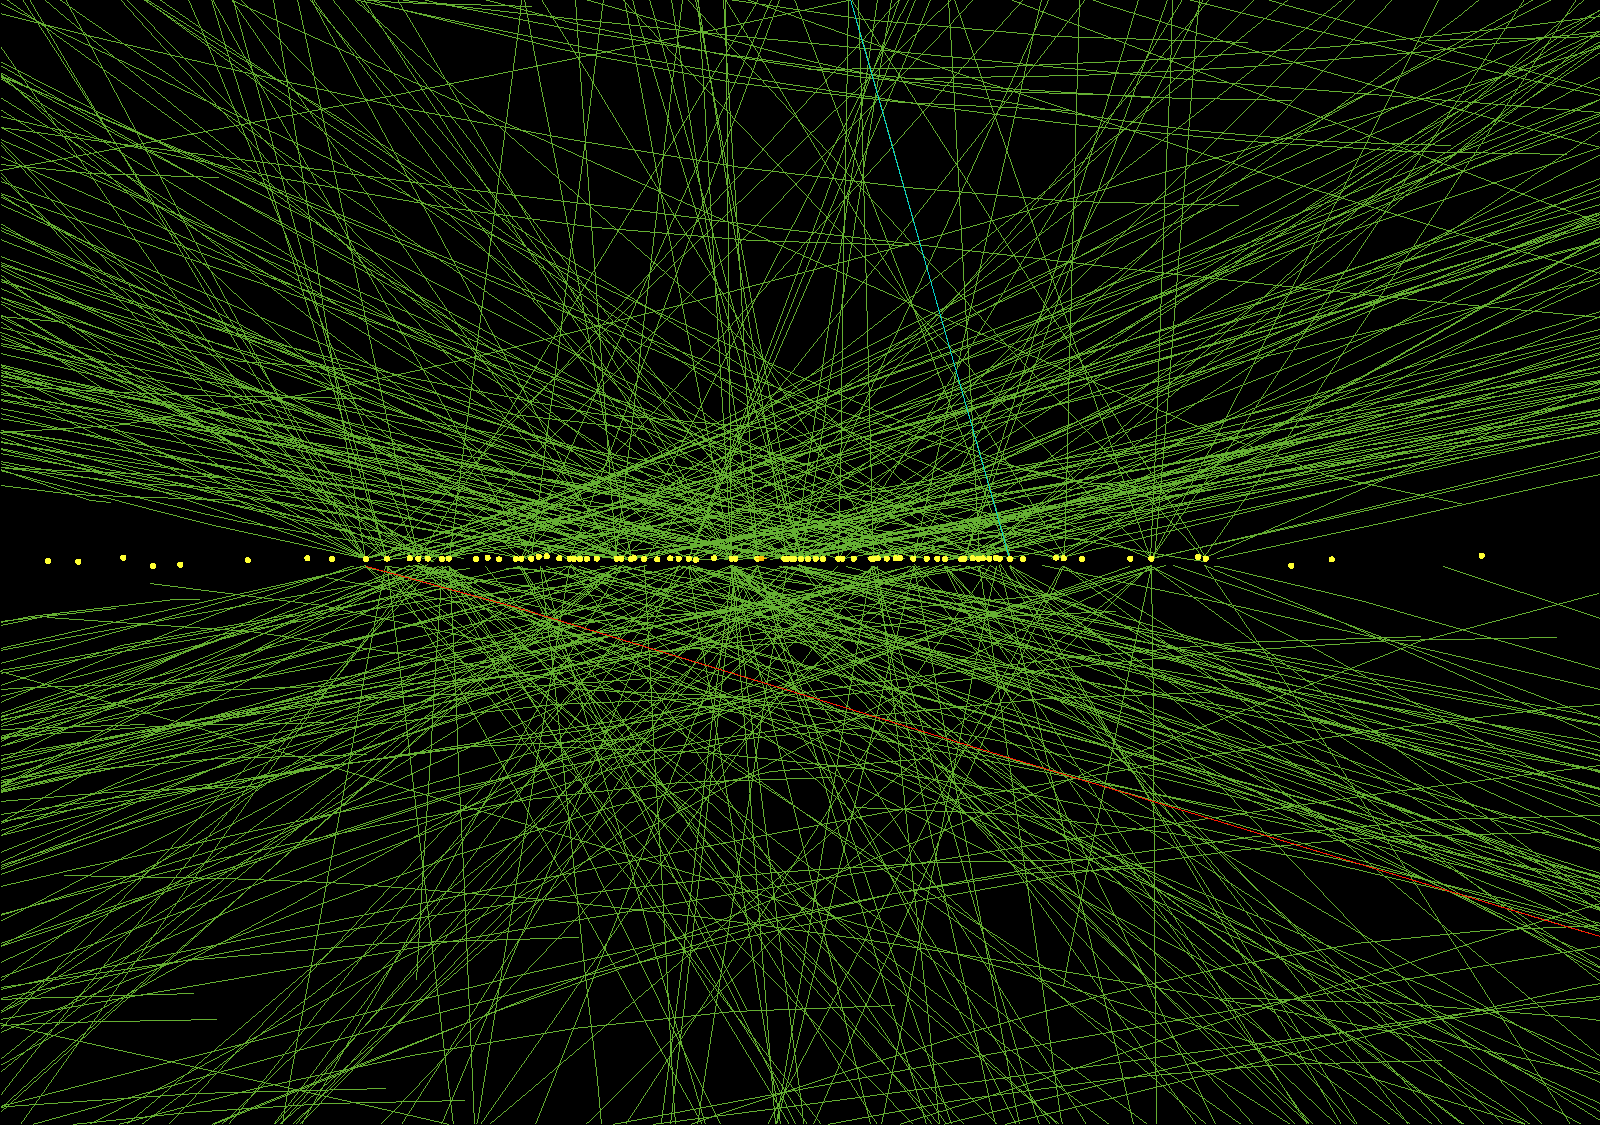
\includegraphics[width=4in]{images/pileup}
    \caption[Event Display of High-Pileup Collision Event]{An event display for a collision from the high-pileup run 198609 which shows 78 reconstructed vertices and their associated charged particle tracks.\cite{pileup}}
    \label{fig:pileup}
\end{figure}

In order to accurately and quickly reconstruct tracks, an iterative tracking algorithm\cite{ITERTRACK} is employed by the CMS experiment which applies several iterations of a combinatorial track finder (CTF) based on Kalman filtering\cite{CMSTRACKRECO} to a collection of hits. Each iteration of the CTF proceeds through the following stages:

\begin{itemize}
  \item \textbf{Seed Generation:} Initial trajectory candidates composed of three hits or two hits and a beamspot or vertex constraint are proposed as seeds.
  \item \textbf{Trajectory Building:} The seeds are extrapolated towards compatible hits in subsequent layers and also towards a single ``invalid'' or fake hit to account for the case where the corresponding hit was not recorded. A Kalman filter then updates the trajectory based on the compatible hit to form track candidates. This extrapolation procedure terminates upon reaching the outermost layer of the tracker or a when ``stop condition'' is satisfied, such as surpassing a maximum number of invalid hits. Because a single seed may produce multiple track candidates and different seeds may produce the same track candidate, an ambiguity resolution based on the fraction of hits shared between pairs of track candidates is applied to prevent double counting.
  \item \textbf{Track Fitting:} The collection of hits for each track candidate is refitted by a Kalman filter and smoother to obtain optimal estimates of the track parameters illustrated in Figure \ref{fig:track_params}: the signed transverse curvature $q\pT$, the polar angle $\cot \theta_{0}$, the azimuthal angle $\phi_{0}$, the longitudinal impact parameter $d_{z}$, and the signed transverse impact parameter $d_{0}$, all of which are defined at the point of closest approach to the beam axis.
\end{itemize}

\begin{figure}[htbp]
  \centering
    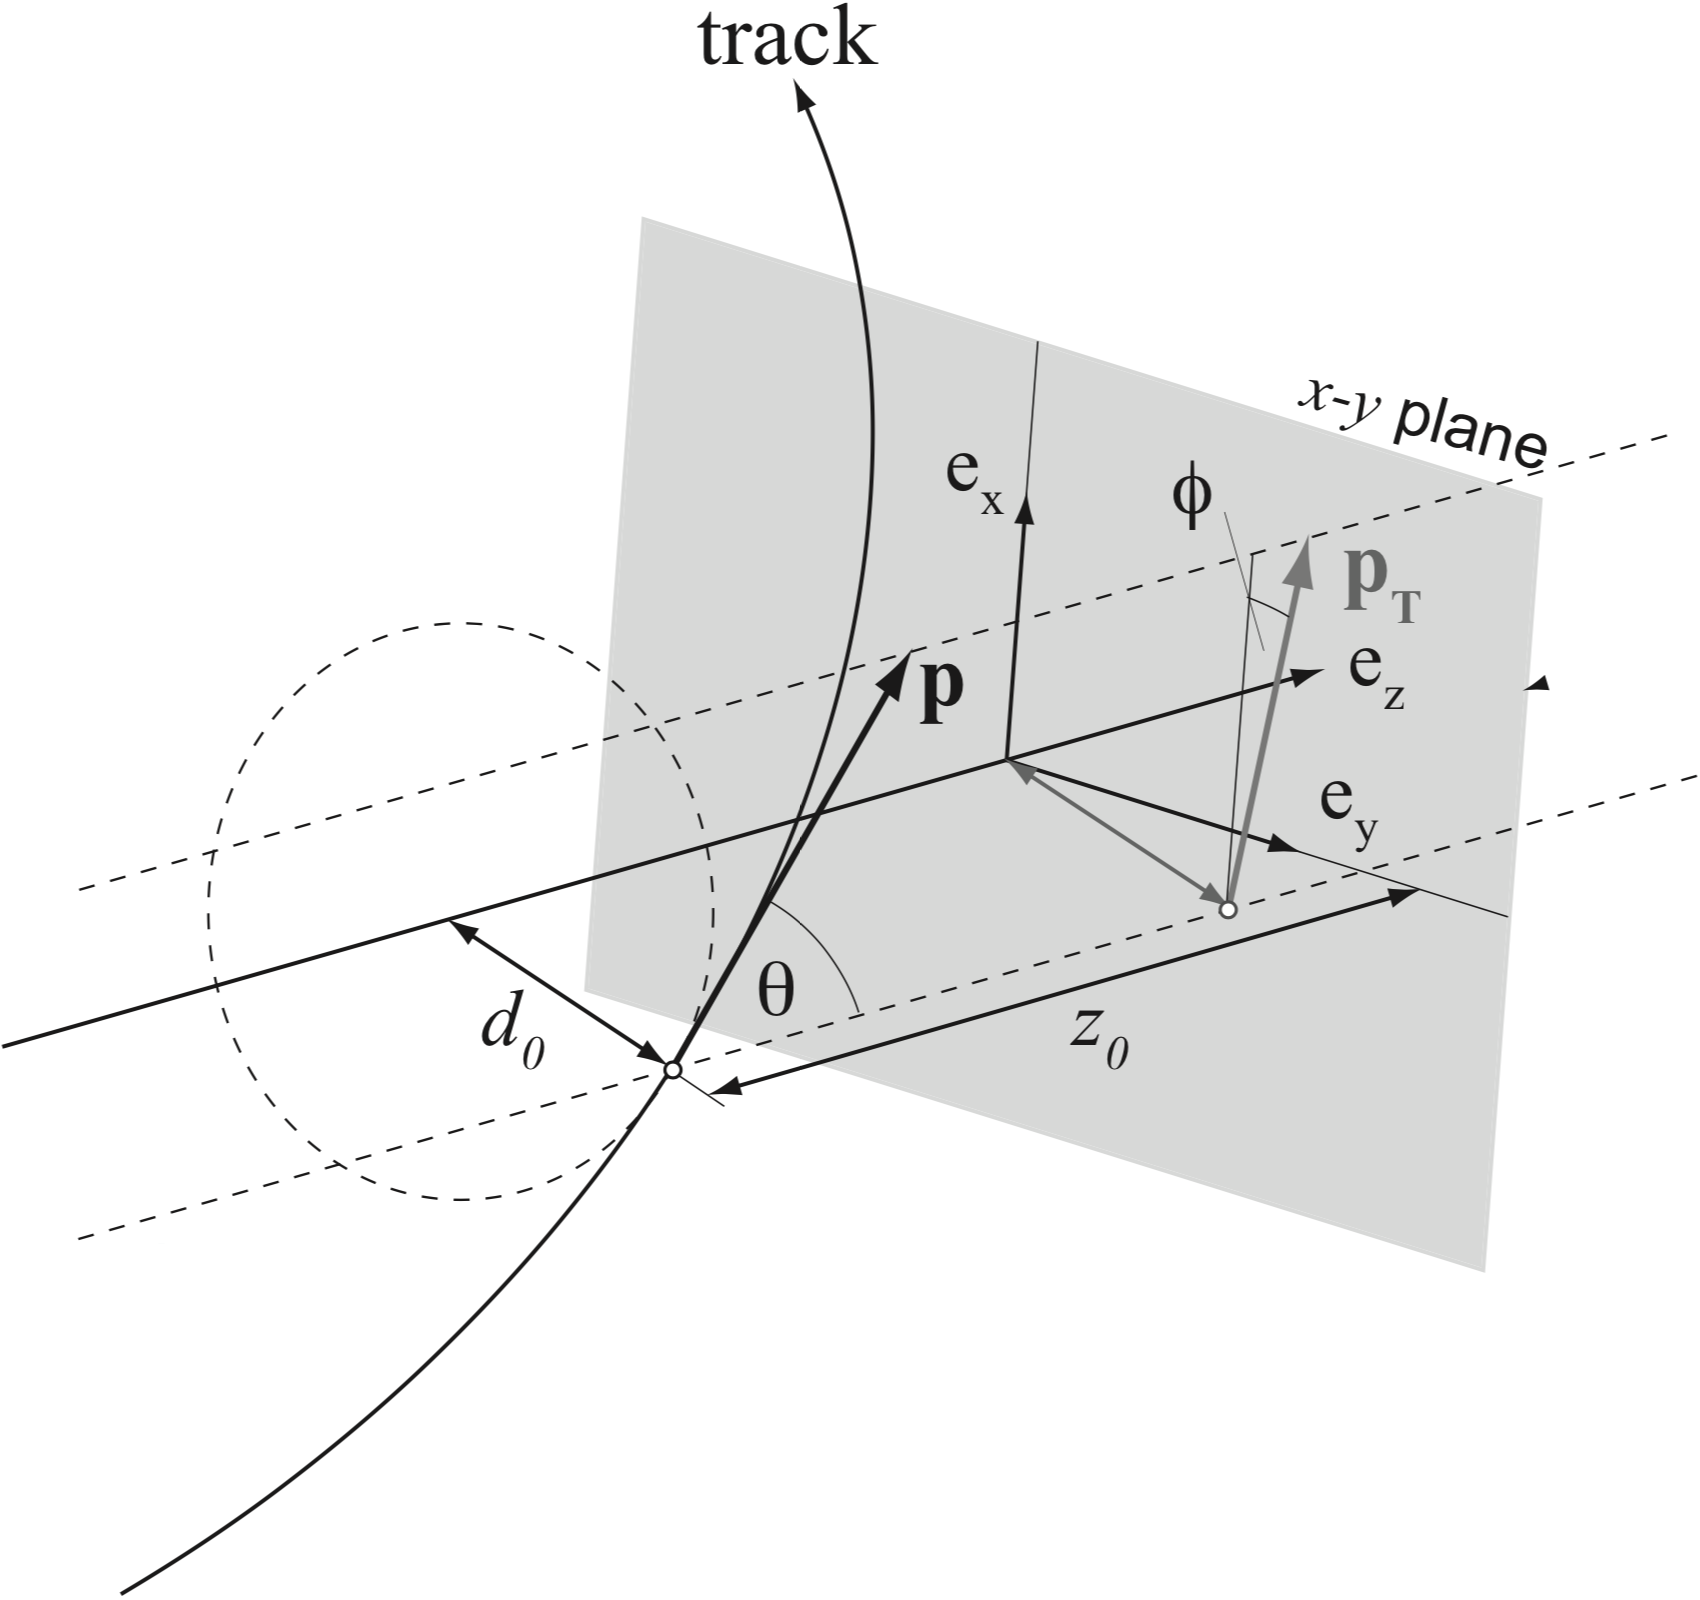
\includegraphics[width=3.5in]{images/track_parameters}
    \caption[Charged Particle Trajectory Parameterization]{The parameterization of a charged particle's trajectory through a magnetic field.\cite{salzburger}}
    \label{fig:track_params}
\end{figure}

The CTF is run for a total of ten iterations in order to achieve a high tracking efficiency while maintaining a near constant misreconstruction rate. The first iteration seeks to reconstruct the easiest tracks which originate close to the interaction point, also called \textit{prompt}, and have high \pT, while the last two iterations attempt to reconstruct muons and will be described in further detail in the subsection \ref{muons}. Because each successive iteration faces increasingly difficult tasks, the hits associated with selected track candidates selected are masked from the subsequent iterations in order to reduce their combinatorial complexity. The seeds and reconstruction targets of the ten iterations are summarized by Table \ref{tbl:itertrack}.

\begin{table}[htbp]
  \caption[Iterative Tracking Summary]{A summary of the ten tracking iterations used by the CMS tracker. The variable $R$ in the final column denotes the distance from the beam axis to the production position of the targeted track.\cite{PARTICLEFLOW}}
  \label{tbl:itertrack}
  \small
  \begin{tabularx}{6.5in}{XXl}
    \hline
    Iteration & Seed Type            & Reconstructed Tracks                    \\
    \hline
    1         & pixel triplets       & prompt, high \pT                        \\
    2         & pixel triplets       & from b hadron decays, $R \lesssim 5$ cm \\
    3         & pixel triplets       & prompt, low \pT                         \\
    4         & pixel pairs          & recover high \pT                        \\
    5         & pixel+strip triplets & displaced, $R \lesssim 7$ cm            \\
    6         & strip triplets/pairs & very displaced, $R \lesssim 25$ cm      \\
    7         & strip triplets/pairs & very displaced, $R \lesssim 60$ cm      \\
    8         & pixel+strip pairs    & inside high \pT jets                    \\
    9         & muon-tagged tracks   & muons                                   \\
    10        & muon detectors       & muons                                   \\
    \hline
  \end{tabularx}
\end{table}

\begin{figure}[htbp]
  \centering
  \mbox{
    \subfigure [] {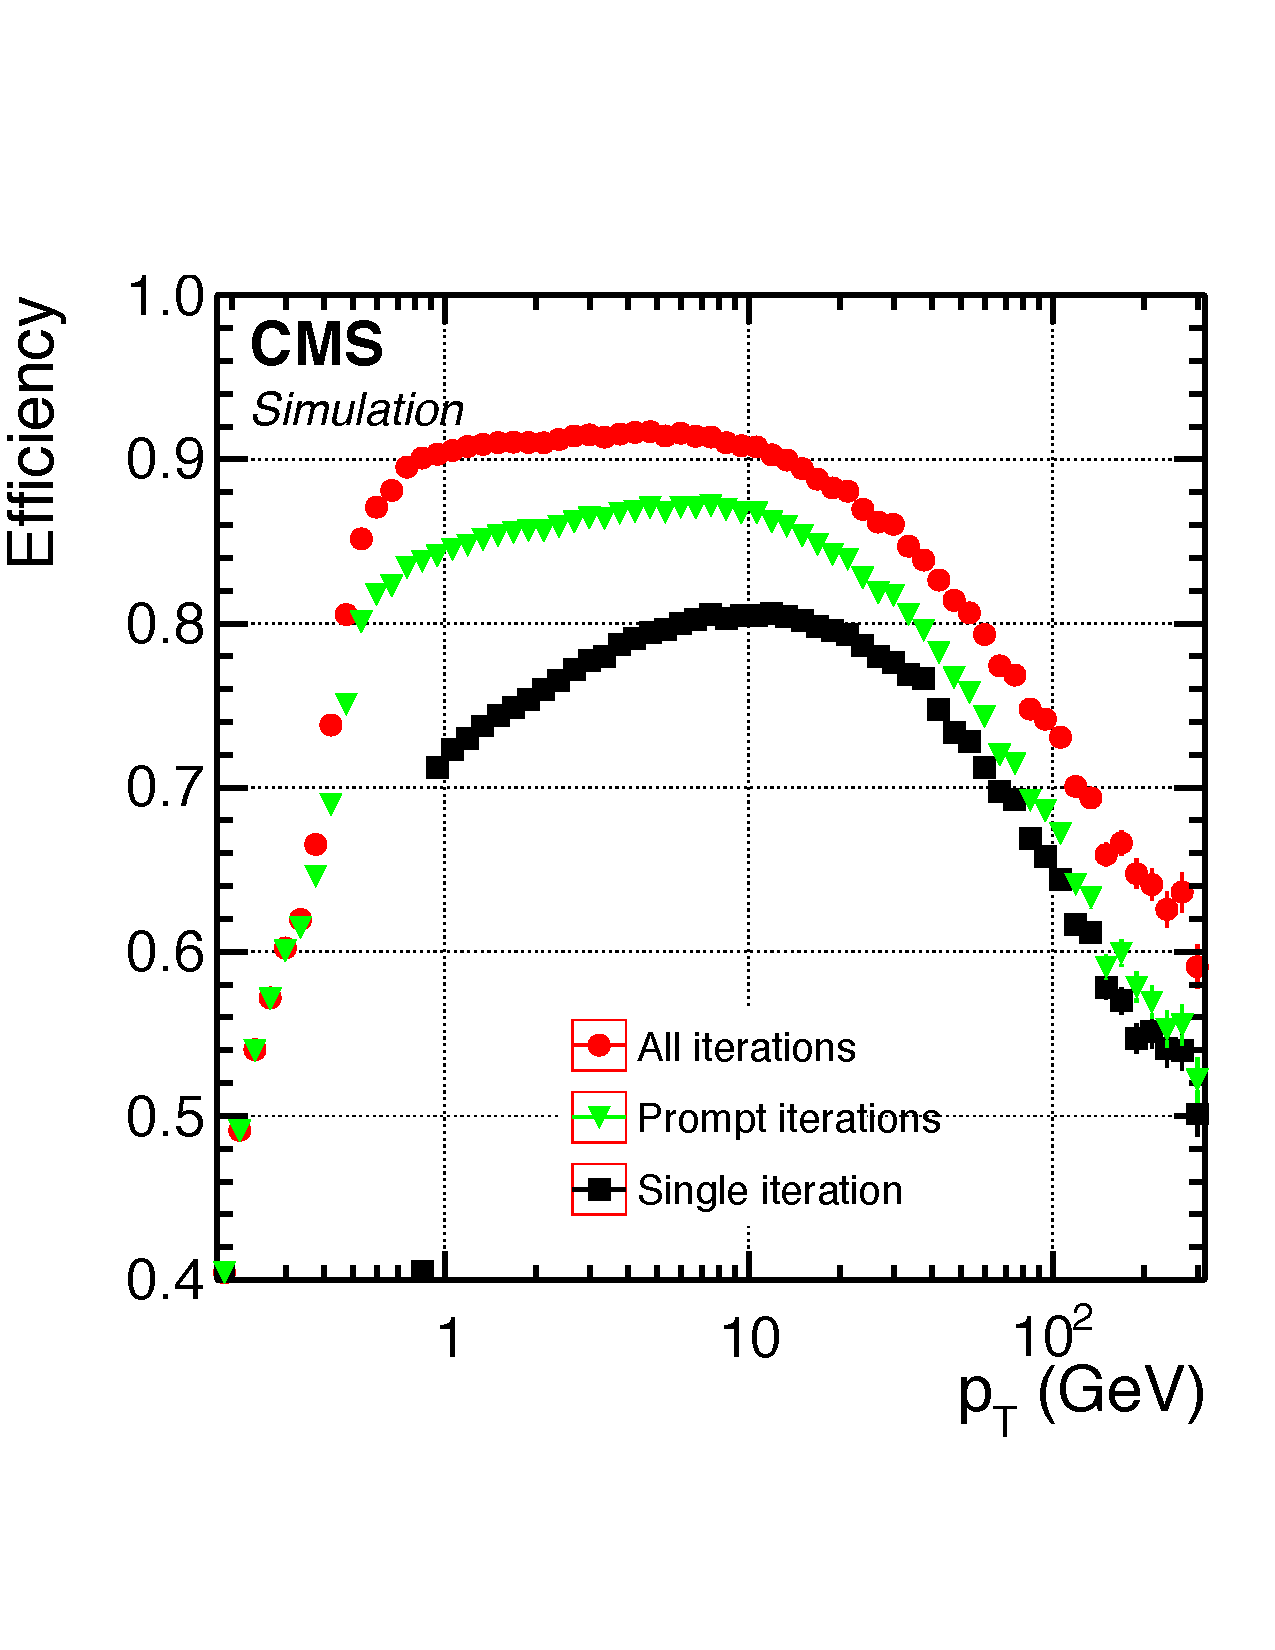
\includegraphics[scale=0.4]{images/pftrack_eff}} \qquad
    \subfigure [] {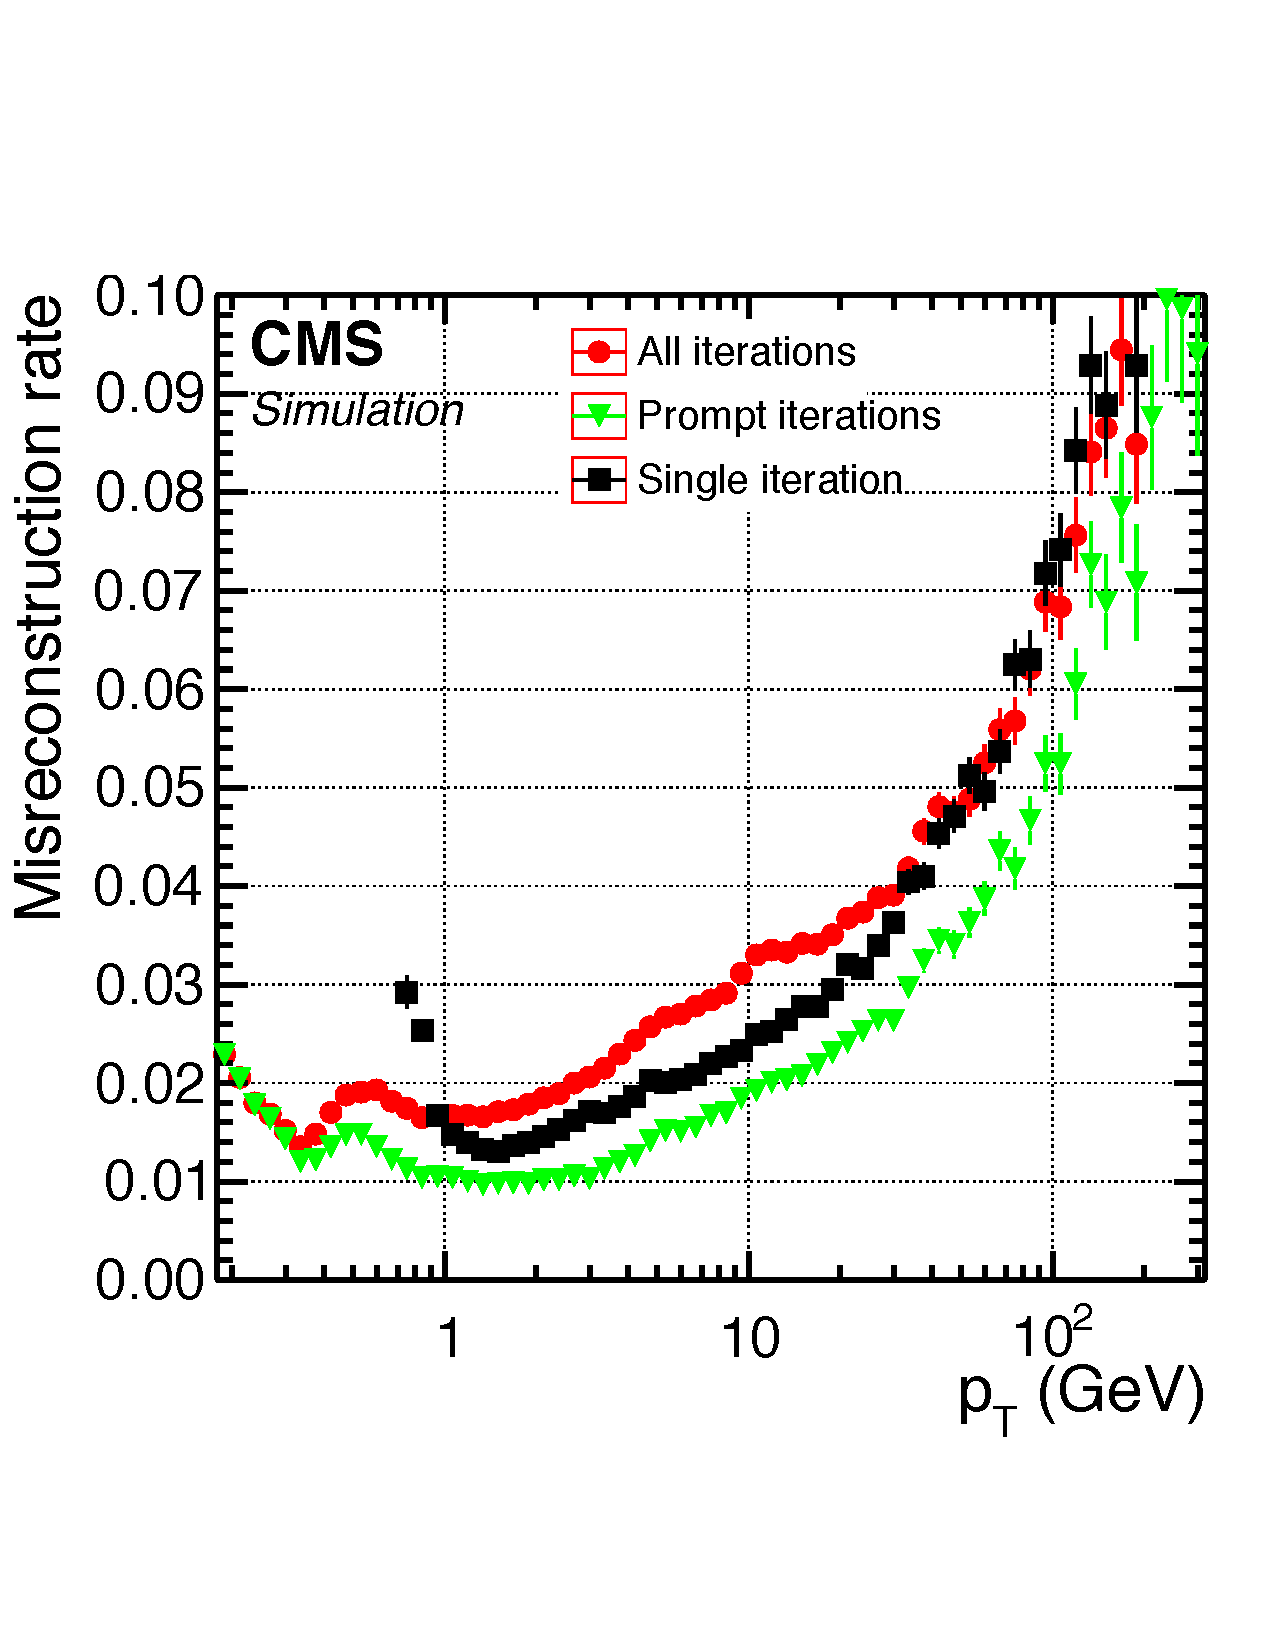
\includegraphics[scale=0.4]{images/pftrack_misreco}} \qquad
  }
  \caption[Track Reconstruction Performance]{The tracking efficiency (A) and misreconstruction rate (B) of charged hadron tracks in simulated multijet events for a single, global iteration of the combinatorial track finder (black squares), the prompt iterations (iterations 1, 2, 3, 4, 5, and 7) of the iterative tracking method (green triangles), and the full iterative tracking method (red circles) as a function of track \pT.\cite{PARTICLEFLOW}}
    \label{fig:pftrack_perf}
\end{figure}

The tracking efficiency and misreconstruction rate are shown in Figure \ref{fig:pftrack_perf}. The full iterative tracking method achieves a 90\% reconstruction efficiency for tracks with \pT\ between 1 \GeV\ and 10 \GeV\, to be compared with the 70-80\% efficiency of the global CTF, and maintains an approximately 8-10\% higher efficiency than the global CTF for tracks with $\pT > 100 \GeV$. Although the iterative tracking method incurs a slightly higher misreconstruction rate than the global CTF, it is able to reconstruct over half of the tracks missed by the global CTF while running twice as fast.

\subsection{Calorimeter Clusters}

\section{Primary Vertices}

\subsection{Pileup Treatment}

\section{Leptons}

\subsection{Electrons}

\subsection{Muons}\label{muons}

\section{Jets}

\subsection{Jet Clustering Algorithms}

\subsection{\qrkb-Tagging}

\section{Missing Transverse Energy}

Additional ``soft'' hadronic activity?

